% SmolVLA on LIBERO, version 2 (10 Nov 2026): lightning talk, NVIDIA Jetson AI Lab Research Group call.
% Build:  tectonic slides_v2.tex      (makes slides_v2.pdf; images and clips come from ../media)
% Numbers: docs/RESULTS_SPEED.md and docs/RESULTS_VOICE.md
\documentclass[aspectratio=169,10pt]{beamer}

\usetheme[progressbar=frametitle, numbering=fraction, sectionpage=none]{metropolis}
\usepackage[sfdefault,lining]{FiraSans}
\usepackage{FiraMono}
\usepackage{booktabs}
\usepackage{tikz}
\usetikzlibrary{calc,positioning,arrows.meta}

% ---------- Colours: white page, burnt-orange headings; in the data, Original = orange and Tuned = blue ----------
\definecolor{ink}{HTML}{1F2328}
\definecolor{muted}{HTML}{6B7280}
\definecolor{faint}{HTML}{D1D5DB}
\definecolor{panel}{HTML}{F6F3F0}
\definecolor{accent}{HTML}{B5541C}
\definecolor{accentrule}{HTML}{ECD2C2}
\definecolor{orig}{HTML}{E07B10}
\definecolor{tuned}{HTML}{1A8FD0}
\definecolor{bad}{HTML}{D64545}
\setbeamercolor{normal text}{fg=ink, bg=white}
\setbeamercolor{frametitle}{fg=accent, bg=white}
\setbeamercolor{progress bar}{fg=accent, bg=accentrule}
\setbeamercolor{block body}{bg=panel, fg=ink}
\setbeamercolor{footline}{fg=muted}
\setbeamertemplate{itemize item}{\color{accent}\footnotesize$\blacktriangleright$}
\setbeamerfont{frametitle}{size=\Large, series=\bfseries}
\makeatletter\setlength{\metropolis@progressinheadfoot@linewidth}{1.2pt}\makeatother  % the orange line under each heading

\newcommand{\Orig}{\textcolor{orig}{\textbf{Original}}}
\newcommand{\Tuned}{\textcolor{tuned}{\textbf{Tuned}}}
\newcommand{\bignum}[1]{{\fontsize{26}{28}\selectfont\bfseries #1}}
\newcommand{\sub}[1]{{\color{muted}#1}}
\newcommand{\hl}[1]{{\color{accent}\bfseries #1}}
\newcommand{\panel}[2]{\begin{beamercolorbox}[wd=#1, sep=2mm, rounded=true]{block body}#2\end{beamercolorbox}}

% A clip inside the PDF: a "Movie" annotation over its poster picture. Okular plays it when clicked;
% other viewers show the poster. #1 width, #2 height, #3 poster, #4 video file
\newcommand{\pdfmovie}[4]{\leavevmode\rlap{\special{pdf:ann width \the\dimexpr#1\relax\space height \the\dimexpr#2\relax\space depth 0pt
  << /Subtype /Movie /T (clip) /Border [0 0 0]
     /Movie << /F (#4) /Aspect [1920 1080] >> /A << /ShowControls true >> >>}}#3}

% Grey line at the bottom of a slide: when and where it was measured.
\newcommand{\foot}[1]{%
  \begin{tikzpicture}[remember picture, overlay]
    \node[anchor=south west, text=muted, font=\tiny, inner sep=0]
      at ($(current page.south west)+(0.45cm,0.25cm)$) {#1};
  \end{tikzpicture}}

\begin{document}

% ---------- 1. Title and agenda ----------
\begin{frame}[plain]
  \vspace{9mm}
  {\fontsize{32}{36}\selectfont\bfseries\color{accent} SmolVLA on LIBERO}\\[2.5mm]
  {\large Faster, more efficient inference, and a voice-to-action pipeline}\\[4mm]
  {\color{accentrule}\rule{\linewidth}{1pt}}\\[4mm]
  {\large\bfseries Sisir Kausthubh} \;{\large\sub{@captof-omuamua}}\\[1mm]
  {\small\sub{Lightning talk \;·\; NVIDIA Jetson AI Lab Research Group \;·\; 10 November 2026}}

  \vfill
  \begin{columns}[T,onlytextwidth]
    \column{0.34\textwidth}
      {\fontsize{22}{24}\selectfont\bfseries\color{accent} 1}\\[0.5mm] {\large Faster inference}
    \column{0.34\textwidth}
      {\fontsize{22}{24}\selectfont\bfseries\color{accent} 2}\\[0.5mm] {\large Original vs Tuned}
    \column{0.30\textwidth}
      {\fontsize{22}{24}\selectfont\bfseries\color{accent} 3}\\[0.5mm] {\large Voice to action}
  \end{columns}
  \vspace{7mm}
\end{frame}

% ---------- 2. Setup ----------
\begin{frame}{Setup}
  \vspace{7mm}
  {\large
  \renewcommand{\arraystretch}{2.0}
  \begin{tabular}{@{}l@{\hspace{9mm}}l@{}}
    \hl{\small HARDWARE} & \textbf{Laptop GPU}: RTX 5090 (Blackwell), 24 GB \sub{\normalsize\; · \; not a Jetson} \\
    \hl{\small ROBOT}    & \textbf{Franka Panda arm}, simulated in LIBERO \sub{\normalsize\; · \; MuJoCo physics} \\
    \hl{\small POLICY}   & \textbf{SmolVLA}, run with LeRobot \sub{\normalsize\; · \; Original and Tuned} \\
    \hl{\small VOICE}    & \textbf{Whisper large-v3-turbo} + \textbf{Qwen3.5-4B} \sub{\normalsize\; · \; speech → command} \\
  \end{tabular}}

  \vspace{7mm}
  {\large Everything runs on this one GPU.}
  \foot{LeRobot main of 6 Nov 2026 + PR \#4634 \;·\; PyTorch 2.15 \;·\; MuJoCo 3.8.1}
\end{frame}

% ---------- 3. Three pillars ----------
\begin{frame}{Three pillars, measured together}
  \vspace{3mm}
  {\large A speed-up only counts if accuracy holds and energy drops.}

  \vspace{7mm}
  \begin{columns}[T,onlytextwidth]
    \column{0.32\textwidth}\centering
      \hl{\small SPEED}\\[2mm] \bignum{111.0 ms}\\[1.5mm] \sub{\small per decision}
    \column{0.32\textwidth}\centering
      \hl{\small ACCURACY}\\[2mm] \bignum{82\%}\\[1.5mm] \sub{\small 328 of 400 episodes succeed}
    \column{0.32\textwidth}\centering
      \hl{\small EFFICIENCY}\\[2mm] \bignum{11.0 J}\\[1.5mm] \sub{\small GPU energy per decision}\\[0.8mm] \sub{\scriptsize = GPU energy counter ÷ decisions}
  \end{columns}

  \vspace{7mm}
  \centering The starting point: \Orig{} SmolVLA, with LeRobot's default settings.\\[1.5mm]
  \sub{400 episodes = 40 LIBERO tasks × 10 starting scenes each}
  \foot{Measured 8 Nov 2026}
\end{frame}

% ---------- 4. Where it started: the pull request ----------
\begin{frame}{Where it started: an open pull request}
  \vspace{1mm}
  \begin{columns}[c,onlytextwidth]
    \column{0.50\textwidth}
      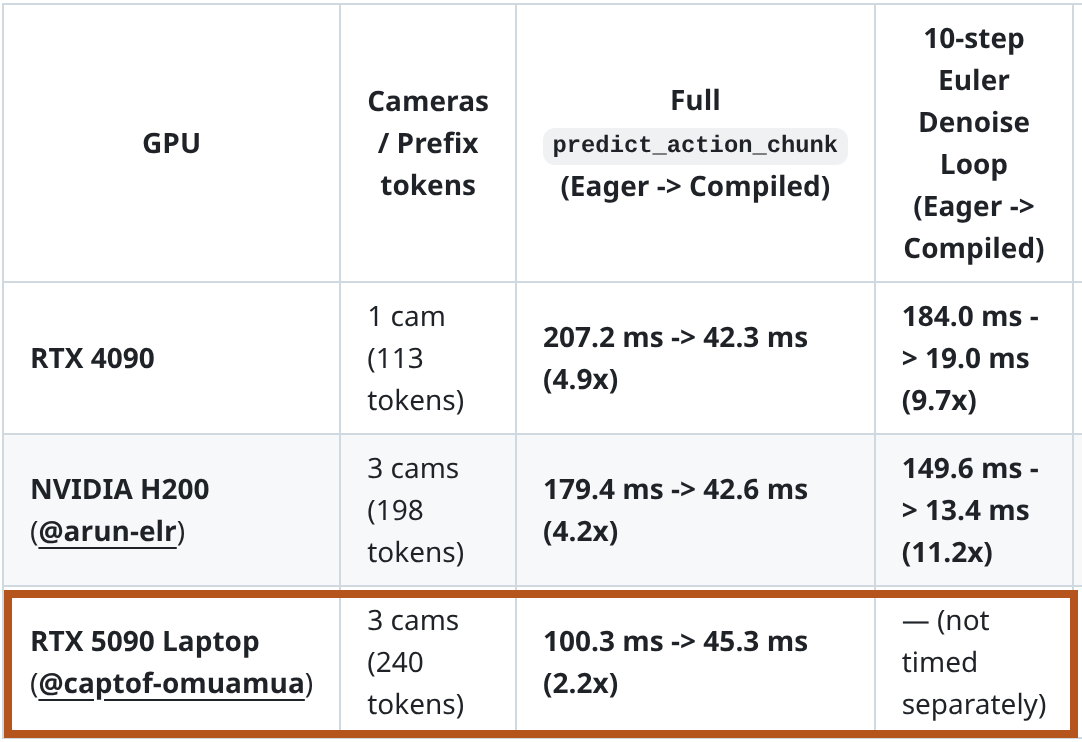
\includegraphics[width=\linewidth]{../media/pr4634_table.png}\\[1mm]
      {\scriptsize\sub{My laptop, the loop alone: 75–79 → 18–19 ms, about 4×. Measured 7 Nov, not posted yet.}}
    \column{0.45\textwidth}
      {\large \hl{PR \#4634} by NotNANtoN (Anton)}\\[0.5mm]
      \sub{\small LeRobot \;·\; still open}

      \vspace{3.5mm}
      SmolVLA reads the scene once, then refines its action in 10 steps.\\[1.5mm]
      The PR keeps that reading fixed \sub{(the KV cache)}, so the 10 steps can be compiled.

      \vspace{3.5mm}
      \begin{tabular}{@{}l@{\hspace{5mm}}r@{}}
        RTX 4090 & 4.9× \\
        H200 & 4.2× \\
        \textbf{My laptop} & \hl{2.2×} \\
      \end{tabular}

      \vspace{3mm}
      I reviewed it and ran it. My numbers are in the table.
  \end{columns}
  \foot{github.com/huggingface/lerobot/pull/4634 \;·\; screenshot of the PR description, 10 Nov 2026}
\end{frame}

% ---------- 5. From 2.2x to 7.7x ----------
% One row of the ladder: #1 height on the page, #2 speed-up factor, #3 colour, #4 label, #5 whose work, #6 the times
\newcommand{\rung}[6]{%
  \node[anchor=south west, inner sep=0] at (0,#1+0.42) {\small #4 \;\sub{\footnotesize #5}};
  \fill[#3] (0,#1) rectangle (#2,#1+0.32);
  \node[anchor=west] at (#2,#1+0.16) {\small\textbf{#2×} \;\sub{\footnotesize #6}};}
\begin{frame}{From 2.2× to 7.7×: what I added}
  \vspace{1mm}
  \begin{columns}[T,onlytextwidth]
    \column{0.60\textwidth}
      \begin{tikzpicture}[x=0.62cm, y=1cm]   % 1× of speed-up = 0.62 cm
        \rung{2.9}{2.2}{muted}{PR \#4634 alone}{10 steps, compiled loop}{100.3 → 45.3 ms}
        \rung{1.5}{4.0}{muted}{1 denoising step, batched cameras}{LeRobot setting + my port}{111.0 → 27.9 ms}
        \rung{0.1}{7.7}{tuned}{\Tuned: plus whole-model compile}{LeRobot's switch}{111.0 → 14.4 ms}
      \end{tikzpicture}

      \vspace{0.5mm}
      {\footnotesize\sub{\Tuned{} = the same model and weights, with faster settings. Nothing was retrained.\\ These two settings also run on plain LeRobot today: 15.4 ms, 7.2×.}}
    \column{0.36\textwidth}
      \bignum{\textcolor{tuned}{7.7×}} \;faster

      \vspace{2.5mm}
      \bignum{\textcolor{tuned}{7.6×}} \;less energy\\[0.3mm] \sub{\small 11.0 → 1.44 J per decision}

      \vspace{2.5mm}
      \bignum{82\%} \;success, both\\[0.3mm] \sub{\small 328 of 400 episodes each}
  \end{columns}

  \vspace{2mm}
  \textbf{The price:} \Tuned{}'s first start takes about 2.5 minutes to compile. \sub{After that, 6.5 s.}
  \foot{Measured 8 Nov 2026, batch 1 \;·\; same 400 starting scenes for both \;·\; PR-alone row: 30 Oct \;·\; plain-LeRobot time: 10 Nov, speed only}
\end{frame}

% ---------- 6. Demo 1: Original against Tuned ----------
\begin{frame}{{\small$\blacktriangleright$}\, Demo 1: Original vs Tuned, same scene}
  \centering
  \vspace{-1mm}
  \pdfmovie{0.75\linewidth}{0.421875\linewidth}{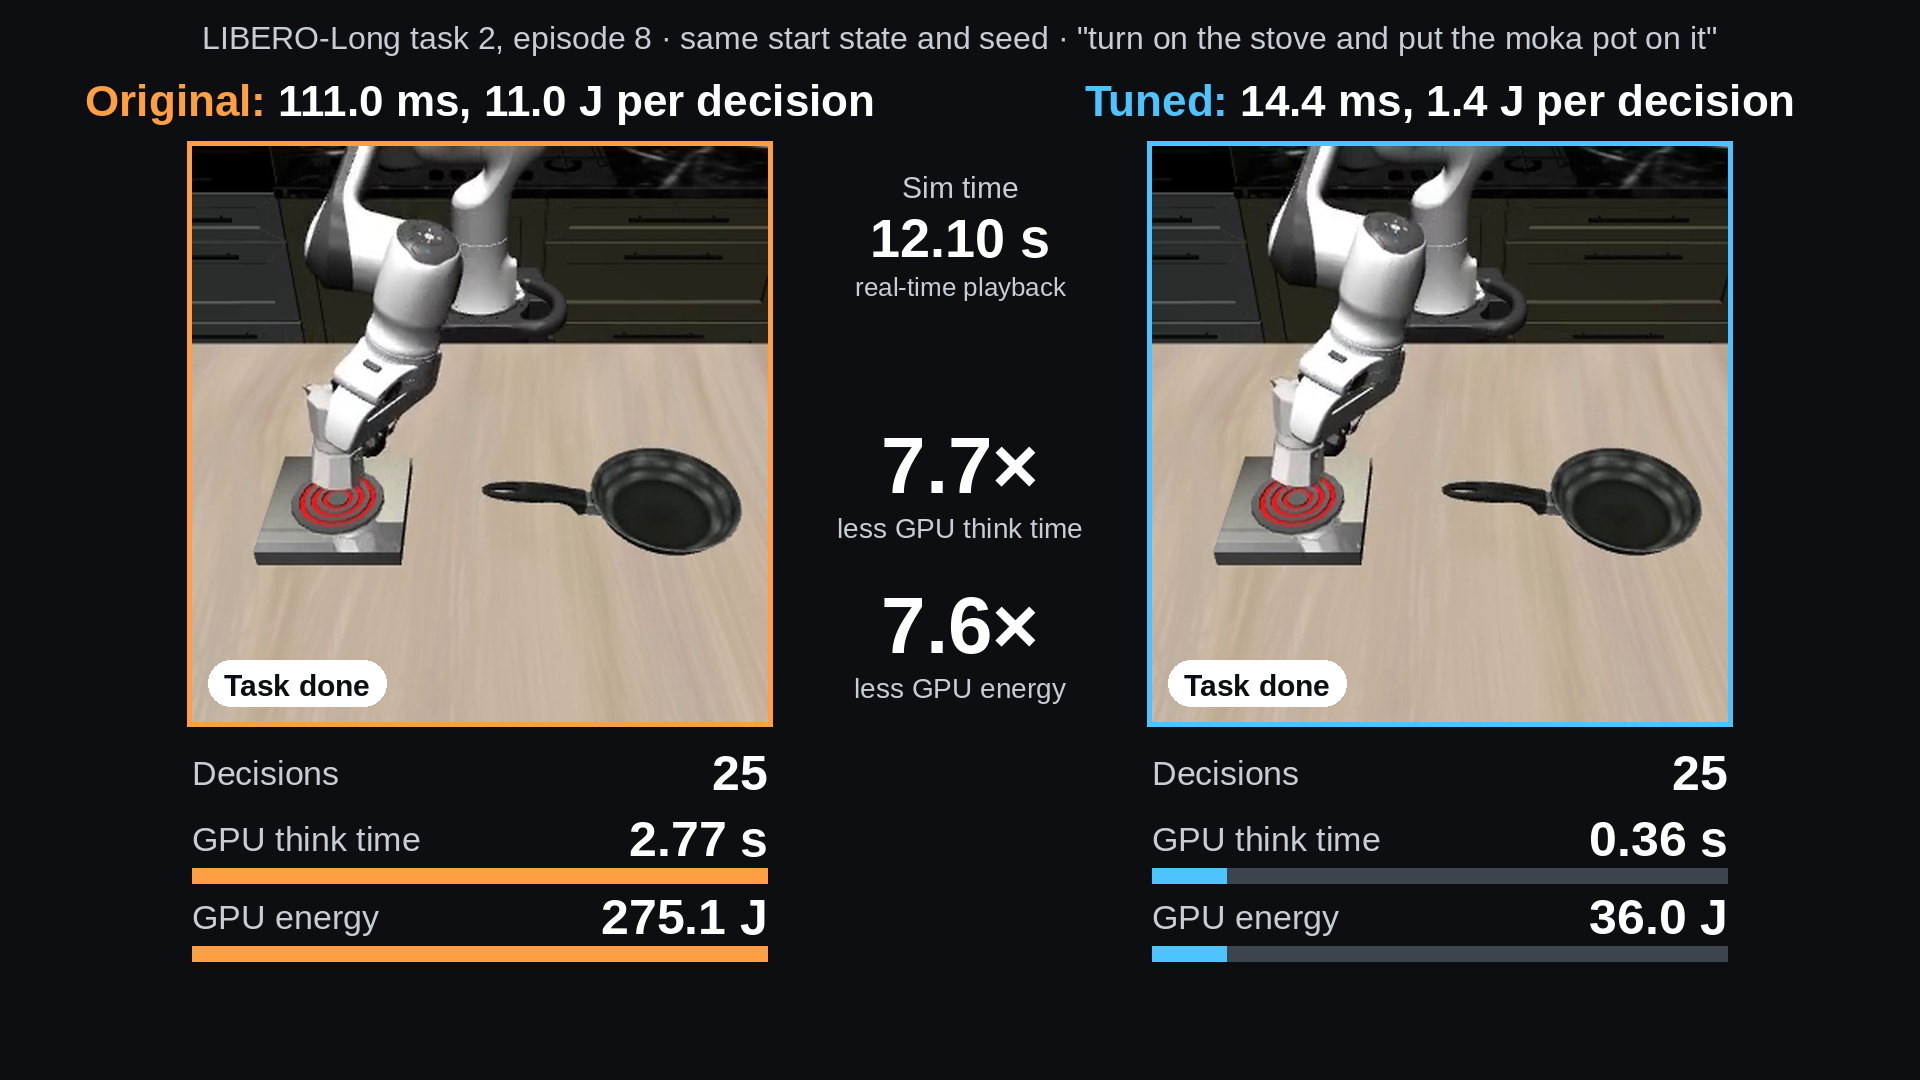
\includegraphics[width=0.75\linewidth]{../media/meters_side_by_side_clean.png}}{../media/meters_side_by_side_clean.mp4}

  \vspace{1.5mm}
  {\small The simulator waits for the model, so both arms move in step. \hl{Watch the counters.}}
  \foot{Counters = decisions so far × the measured time and energy per decision \;·\; measured 8 Nov 2026}
\end{frame}

% ---------- 7. Voice to action: the pipeline ----------
% One box of the flowchart: #1 position name, #2 where, #3 label, #4 note under it
\newcommand{\stage}[4]{\node[draw=accentrule, line width=0.8pt, rounded corners=2pt, fill=panel, minimum height=10mm, minimum width=21mm,
    align=center, font=\small\bfseries] (#1) at #2 {#3};
  \node[below=1mm of #1, font=\scriptsize, text=muted, align=center] {#4};}
\begin{frame}{Voice to action: the pipeline}
  \centering
  \vspace{2mm}
  \begin{tikzpicture}[>={Stealth[length=2.2mm]}]
    \stage{v}{(0,0)}{Your voice}{a spoken line}
    \stage{w}{(2.85,0)}{Whisper}{large-v3-turbo\\ speech to text, 60 ms}
    \stage{r}{(5.7,0)}{Router}{picks one of 10 commands\\ Qwen3.5-4B when unsure}
    \stage{p}{(8.75,0)}{SmolVLA, \textcolor{tuned}{Tuned}}{decides every 0.5 s\\ 13 ms per decision}
    \stage{a}{(11.75,0)}{Franka arm}{in LIBERO}
    \foreach \x/\y in {v/w, w/r, r/p, p/a} \draw[->, line width=0.9pt, color=muted] (\x) -- (\y);
  \end{tikzpicture}

  \vspace{5mm}
  {\small
  \begin{tabular}{@{}l@{\hspace{6mm}}l@{}}
    \hl{A command}        & goes to SmolVLA as one of its 10 trained sentences \\[0.6mm]
    \hl{Two commands}     & run in order; the arm returns to its ready pose in between \\[0.6mm]
    \hl{Stop / continue}  & the arm holds, then resumes \\[0.6mm]
    \hl{Anything else}    & refused: the robot does nothing \\
  \end{tabular}}

\end{frame}

% ---------- 8 to 10. Demo 2: three clips with the recorded voice ----------
% One demo slide: #1 title, #2 poster picture, #3 clip file, #4 the numbers on the right, #5 small print
\newcommand{\demoslide}[5]{%
\begin{frame}{#1}
  \vspace{-1mm}
  \begin{columns}[c,onlytextwidth]
    \column{0.60\textwidth}
      \pdfmovie{\linewidth}{0.5625\linewidth}{\includegraphics[width=\linewidth]{../media/#2}}{../media/#3}
    \column{0.36\textwidth}
      #4
  \end{columns}
  \foot{#5}
\end{frame}}

\demoslide{{\small$\blacktriangleright$}\, Demo 2a: one spoken command}{voice_single_poster.png}{take2_single_stove.mp4}{%
  \bignum{3 of 3} \;runs\\[0.3mm] \sub{\small this command, on 3 starting scenes}

  \vspace{3.5mm}
  \bignum{0.2 s}\\[0.3mm] \sub{\small from the last word to the first move}

  \vspace{3.5mm}
  \bignum{3.9 s}\\[0.3mm] \sub{\small of movement to finish, in this run}}
  {My recorded voice, played into the running system \;·\; simulator \;·\; 10 Nov 2026}

\demoslide{{\small$\blacktriangleright$}\, Demo 2b: stop and continue}{voice_stop_poster.png}{take2_stop_continue_stove.mp4}{%
  \bignum{9 of 9} \;runs\\[0.3mm] \sub{\small finish after ``stop'', then ``continue''}

  \vspace{3.5mm}
  \bignum{5–10 mm}\\[0.3mm] \sub{\small overrun after ``stop'', then the arm holds}

  \vspace{3.5mm}
  \bignum{190 ms}\\[0.3mm] \sub{\small from the end of the word to the hold}}
  {Recorded voice, simulator \;·\; 3 commands × 3 starting scenes \;·\; the arm then holds within about 5 mm \;·\; a live microphone would add time to detect the end of speech}

\demoslide{{\small$\blacktriangleright$}\, Demo 2c: two commands in one sentence}{voice_two_step_poster.png}{take2_two_step_drawer_then_stove.mp4}{%
  \bignum{5 of 5} \;runs\\[0.3mm] \sub{\small both done, for this sentence}

  \vspace{3.5mm}
  {\small The arm returns to its ready pose between the two commands.}}
  {Recorded voice, simulator \;·\; this sentence on 5 starting scenes \;·\; 10 Nov 2026}

\demoslide{{\small$\blacktriangleright$}\, Demo 2d: a misheard word is refused}{voice_refusal_poster.png}{refusal_bowl_heard_as_ball.mp4}{%
  {\large I said ``bowl''.\\[1mm] It heard ``ball''.}

  \vspace{4mm}
  \bignum{3 of 3} \;tries\\[0.3mm] \sub{\small refused: no command has a ball}

  \vspace{3.5mm}
  \bignum{0.35 mm}\\[0.3mm] \sub{\small arm movement in the next 3 s}}
  {My recorded voice, played into the running system \;·\; simulator \;·\; 10 Nov 2026}

% ---------- 11. The end ----------
\begin{frame}[plain]
  \vspace{26mm}
  {\fontsize{40}{44}\selectfont\bfseries\color{accent} Thank you}\\[6mm]
  {\color{accentrule}\rule{\linewidth}{1pt}}\\[6mm]
  {\Large\bfseries Sisir Kausthubh} \;{\Large\sub{@captof-omuamua}}
\end{frame}

\end{document}
